% Vorlage für die VWA. Version 20180117 (c) Leonard Michlmayr

% TODO: Wähle den für deine Arbeit die passenden Optionen!
\documentclass[DLS,
	inreferencehack,
	ohneVgl=true,
	ohneS=false,
	noscauthor,
	rundeauslassung=false,
	bookstyle=false,
	widowlines=3]{vwa}

%% Chapter Style
\usepackage{graphicx}
\usepackage{titlesec}

\newcommand*\HUGE{\Huge}
\newcommand*\chapnamefont{\normalfont\LARGE\MakeUppercase}
\newcommand*\chapnumfont{\normalfont\HUGE}
\newcommand*\chaptitlefont{\normalfont\HUGE\bfseries}

\newlength\beforechapskip
\newlength\midchapskip
\setlength\midchapskip{\paperwidth}
\addtolength\midchapskip{-\textwidth}
\addtolength\midchapskip{-\oddsidemargin}
\addtolength\midchapskip{-1in}
\setlength\beforechapskip{18mm}

\titleformat{\chapter}[display]
  {\normalfont\filleft}
  {{\chapnamefont\chaptertitlename}%
    \makebox[0pt][l]{\hspace{.8em}%
      \resizebox{!}{\beforechapskip}{\chapnumfont\thechapter}%
      \hspace{.8em}%
      \rule{\midchapskip}{\beforechapskip}%
    }%
  }%
  {25pt}
  {\chaptitlefont}
\titlespacing*{\chapter}
  {0pt}{40pt}{40pt}

%% Abkürzungen
\newcommand{\zB}{z.\,B. }
\newcommand{\ua}{u.\,a. }
\newcommand{\dH}{d.\,h. }

%% Trick texlipse to use biber instead of bibtex
\iffalse
\usepackage[error,backend=biber]{biblatex}
\fi
%%

\usepackage{textcomp}
\usepackage[output-decimal-marker={,}]{siunitx}
\usepackage{tabularx}
\usepackage{booktabs}
\usepackage{acronym}

\usepackage{amsmath}
\DeclareMathOperator{\arctantwo}{arctan2}

\usepackage{array}
\newcolumntype{P}[1]{>{\centering\arraybackslash}p{#1}}

\renewcommand{\autodot}{}

% TODO: Link visit date aktualisieren
\addbibresource{quellen.bib}
\graphicspath{{img/}}

\Autor{Martin Sonnberger}
\Klasse{8C}
\Betreuer{Mag. Leonard Michlmayr}
\Thema{Positionsbestimmung beim autonomen Fahren}

% TODO: erst bei der letzten Version das Abgabedatum anführen
%\Abgabedatum{}

\begin{document}

% Am Anfang keine Seitennummern
\frontmatter

% PDF-Lesezeichen für die Titelseite
\pdfbookmark[0]{Titelseite}{titlepage}
% Titelseite
\maketitle

% TODO: Abstract einfügen
% \addchap{Abstract}

In dieser vorwissenschaftlichen Arbeit wird der Prozess des autonomen Fahrens genauer erläutert. Insbesondere wird die Frage beantwortet, welche Methoden angewandt werden, um die Position eines autonomen Fahrzeugs präzise bestimmen zu können.
\bigskip

Im ersten Teil der Arbeit wird der Begriff des autonomen Fahrens und die verschiedenen Stufen, in die die Autonomie eines Fahrzeugs eingeteilt werden kann, erklärt. Außerdem werden die im Fahrzeug verbauten Sensoren sowie der Prozess des autonomen Fahrens behandelt. Fortgesetzt wird die Arbeit mit den verschiedenen Methoden der Lokalisierung, abschließend wird der aktuelle Entwicklungsstand, sowohl von Produkten zur Positionsbestimmung als auch von Projekten zum autonomen Fahren, dargelegt.
\bigskip

Nach intensiver Auseinandersetzung mit dem Thema habe ich die Erkenntnis gewonnen, dass noch keine der in dieser Arbeit behandelten Technologien eine endgültige Lösung für das Problem der notwendigen genauen Positionsbestimmung darstellt. Letztendlich müssen die Fahrzeughersteller wohl auf eine Kombination verschiedener Systeme zurückgreifen, um den hohen Anforderungen gerecht zu werden.


% TODO: eventuell Vorwort einfügen
% \include{vorwort}

% Das Inhaltsverzeichnis soll ein PDF-Lesezeichen aber keinen Eintrag im
% Inhaltsverzeichnis haben.
\cleardoublepage\pdfbookmark[0]{\contentsname}{toc}
% Inhaltsverzeichnis
\tableofcontents

% Hier geht es los.
\mainmatter

\chapter{Autonomes Fahren --- Beschreibung allgemein}

Versucht man den Begriff \enq{Autonomes Fahren} zu definieren, stößt man unweigerlich auf das Automobil und dessen Erfindung im Jahr 1886. Der Begriff \enq{Automobil} setzt sich aus dem griechischen \textit{autòs} (\enq{selbst}) und dem lateinischen \textit{mobilis} (\enq{beweglich}) zusammen, bedeutet also \enq{Selbstbewegliche}. Damals sollte dadurch die von nun an bestehende Unabhängigkeit von Kutschpferden verdeutlicht werden. Genauer betrachtet fällt auf, dass durch das Wegfallen von Pferden die Autonomie in gewisser Weise verloren ging. Durch jahrelanges Training konnten sich die Pferde in Maßen selbst fortbewegen, indem sie beispielsweise einen nicht mehr fahrtüchtigen Kutscher alleine nachhause brachten.
\vgl[2-3]{Maurer}
Durch die Einführung von zahlreichen Fahrerassistenzsystemen und letzendlich des autonomen Fahrens wird dem Automobil seine ursprünglich gedachte Autonomie nicht nur wieder zurückgegeben, sondern auch um ein Vielfaches erweitert.


\section{Begriffsdefintion}

\dzit{Definition}{Autonomes Fahren bedeutet das selbständige, zielgerichtete Fahren eines Fahrzeugs im realen Verkehr, ohne Eingriff des Fahrers.}

Autonomes Fahren beschreibt die Übergabe aller mit der Fahrzeugführung verbundenen Tätigkeiten wie beschleunigen, bremsen, lenken, etc., an eine Maschine, den sogenannten Fahrroboter, welcher selbstständig, ohne Mitwirken des Menschen, Entscheidungen trifft. Dabei darf von autonomen Fahrzeugen keine größere Gefahr, als von Menschen gesteuerten ausgehen. Primäre Informationsquellen sind visuelle Quellen, wie sie auch dem Fahrer zur Verfügung stehen.
\vgls[667]{Winner}{Definition}

Ein Punkt, in dem sich autonom gesteurte Fahrzeuge von heutigen Maschinen unterscheiden, ist die Unvorhersehbarkeit ersterer. Maschinen im heutigen Alltag werden entweder von Menschen gesteuert (\zB Autos, Baumaschinen), oder führen stark eingeschränkte, sich wiederholende Bewegungen durch (\zB Aufzüge, Rolltreppen). Autonome Fahrzeuge hingegen bewegen sich auf normalen Straßen und fahren auf beinahe allen Wegen, die auch ein menschlicher Fahrer benutzen würde. Zusammen mit der alleinig durch den Computer stattfindenden Entscheidungsfindung, lässt sie das in ihren Entscheidungen unvorhersehbar machen.

Selbstfahrende Autos stellen eine neue Klasse an von Computern kontrollierten Systemen dar, in der die Maschine Entscheidungen für sich selbst trifft. Um solche Systeme zu verstehen, ist es umso wichtiger, ein Verständnis der dahintersteckenden Technologie von autonomen Fahrzeugen zu haben. Einer Technologie, die es ihnen erlaubt, sich selbst durch das komplexe Straßennetz zu manövrieren.
\vgl[130]{Surden}

\subsection{Autonomiestufen}
Der Grad der Automatisierung eines Fahrzeugs kann in verschiedene Stufen eingeteilt werden, welche Autonomiestufen oder Level genannt werden. Eine erste Einteilung in fünf Stufen erfolgte 2013 in den USA von der \ac{NHTSA}. Im Jahr 2014 veröffentlichete die \ac{SAE} zum ersten Mal den J3016-Standard, welcher eine Überarbeitung der ursprünglichen Einteilung der \ac{NHTSA} darstellt. Der Hauptgrund für die Adaptierung war die Standardisierung verschiedener Skalen. Der größte Unterschied besteht in einer zusätzlichen, sechsten Stufe, die für die Einteilung verwendet wird. \vgl[11-13]{Kaufleitner} Der J3016-Standard ist die heute am weitesten verbreitete Einteilung, auch das \ac{bmvit} verwendet ihn als Grundlage. (H.~Atasayar, persönliche Kommunikation, 20. Aug. 2018)

Am Beginn der Skala steht Level 0, was bedeutet, dass sämtliche Fahraufgaben durch den Menschen erfolgen. Level 5 hingegen steht für eine vollständige Automation, bei der jegliche, für eine Fahrt erforderlichen Aufgaben, durch den Computer ausgeführt werden. Bei Begriffen wie \enq{selbstfahrend}, \enq{fahrerlos} oder auch \enq{autonom}, ist meist von einer vollständigen Automation auf Level 5 die Rede.

In der Zusammenfassung der Autonomiestufen (\ref{levels}) ist oft von der \textit{Dynamischen Fahraufgabe} die Rede, die \ac{SAE} definiert sie folgendermaßen: \zit[6]{sae-j3016}{All of the real-time operational and tactical functions required to operate a vehicle in on-road traffic, excluding the strategic functions such as trip scheduling and selection of destinations and waypoints \elp{}}

%TODO: Fragen ob das stimmt
\nocite{wiki-levels}
\begin{table}[p]
    \begin{tabularx}{\textwidth}{P{1.2cm}lX}
      \toprule

      \textbf{SAE Level} & \textbf{Name} & \textbf{Definition} \\

      \midrule
      \multicolumn{3}{l}{Menschlicher Fahrer kontrolliert die Umgebung.} \\
      \midrule

      0 & Keine Automation & die durchgängige Ausführung aller Aspekte der dynamischen Fahraufgabe durch den menschlichen Fahrer, auch wenn unterstützende Warn- oder Interventionssysteme eingesetzt werden. \\[0.3cm]

      1 & Fahrerassistenz & eine Fahrer-Assistenz, die Fahrmodus-spezifische Aufgaben wie die Lenk-Assistenz oder Beschleunigungs- /Brems-Assistenz dank der Verwendung von Fahr- und Umgebungsinformationen ausführt und mit der Erwartung, dass der menschliche Fahrer alle verbleibenden Aspekte der dynamischen Fahraufgabe ausführt \\[0.3cm]

      2 & Teilautomation & die Fahrmodus-spezifische Ausführung von Lenk- und Beschleunigungs- /Bremsvorgängen durch ein oder mehrere Fahrerassistenzsysteme unter Verwendung von Informationen über die Fahrumgebung und mit der Erwartung, dass der menschliche Fahrer alle verbleibenden Aspekte der dynamischen Fahraufgabe ausführt \\

      \midrule
      \multicolumn{3}{l}{Das System kontrolliert die Umgebung.} \\
      \midrule

      3 & Bedingte Automation & die Fahrmodus-spezifische Ausführung aller Aspekte der dynamischen Fahraufgabe durch ein automatisiertes Fahrsystem mit der Erwartung, dass der menschliche Fahrer auf Anfrage des Systems angemessen reagieren wird \\[0.3cm]

      4 & Hohe Automation & die Fahrmodus-spezifische Ausführung aller Aspekte der dynamischen Fahraufgabe durch ein automatisiertes Fahrsystem, selbst wenn der menschliche Fahrer auf Anfrage des Systems nicht angemessen reagiert \\[0.3cm]

      5 & Volle Automation & die durchgängige Ausführung aller Aspekte der dynamischen Fahraufgabe durch ein automatisiertes Fahrsystem unter allen Fahr- und Umweltbedingungen, die von einem menschlichen Fahrer bewältigt werden können \\

      \bottomrule
    \end{tabularx}
  \caption[Einteilung der Autonomiestufen nach SAE J3016. Quelle: \fullcite{sae-j3016}.]{Einteilung der Autonomiestufen nach SAE J3016 (\quotecite(vgl.)()[19]{sae-j3016}[]{wiki-levels})}
  \label{levels}
\end{table}



\section{Technologie von autonomen Fahrzeugen}

%TODO: Sekundärzitat: Quelle finden!
Bei einem hohen Automatisierungsgrad wird die Technologie verwendet, um die folgenden drei primären Fragen zu beantworten: \vgl[137]{Surden}
\begin{enumerate}
  \item{Wo befindet sich das Fahrzeug?}
  \item{Welche Objekte befinden sich um das Fahrzeug herum?}
  \item{Wo ist es gewünscht, erlaubt und sicher, sich als nächstes hinzubewegen?}
\end{enumerate}
Einem autonomen Fahrzeug muss es möglich sein, diese Fragen unter Berücksichtung von Verkehrszeichen, Ampeln und Straßenmarkierungen, zu beantworten. Außerdem muss es in einem Raum voll mit Objekten wie Fahrzeugen, Fußgängern, Radfahrern und Tieren, sicher navigieren können. Um diese Aufgaben erfolgreich zu bewältigen, ist ein Zusammenspiel von \textbf{Hardware} und \textbf{Software} notwendig.

\subsection{Sensoren}
In autonomen Fahrzeugen sind zahlreiche Sensoren installiert, die dazu beitragen, alle drei oben genannten Fragen, zu beantworten. Sensoren sind Komponenten, die eine physikalische Größe der Umgebung oder des Fahrzeuges selbst in ein elektrisches Signal umwandeln, welches an den Fahrzeugcomputer weitergeleitet wird, um es dort weiterzuverarbeiten. \vgl{sensor-def} In autonomen Fahrzeugen wird meist ein \acs{Radar} (\acl{Radar}) verwendet, um Hindernisse zu erkennen, sowie deren Entfernung und Geschwindigkeit zu bestimmen. Dazu werden elektromagentische Wellen im Frequenzbereich der Mikrowellen (meist \SI{24}{\giga\hertz}) ausgesendet. Treffen sie auf ein Objekt, werden die Wellen reflektiert und vom Empfänger des \acs{Radar}, welcher meist gleichzeitig auch den Sender darstellt, aufgefangen. Mithilfe des gemessenen Zeitunterschiedes können nun Entfernung und Geschwindigkeit des Objekts berechnet werden. \vgl{sensors-thedrive}

Ein weiterer, bereits in heutigen, konventionellen Fahrzeugen eingesetzter Sensor, ist der Ultraschallsensor. Aufgrund seiner Beschränkungen in Hinsicht auf Reichweite und Maximalgeschwindigkeit ist er jedoch nicht so vielseitig anwendbar wie ein \acs{Radar}. Wegen seiner Kompaktheit sowie kostengünstigen Herstellung ist er jedoch besonders bei Einparksystemen beliebt.

Mithilfe von \acs{Lidar}-Scannern (\acl{Lidar}), ist es möglich, nicht nur Objekte an sich, sondern auch um welche Art von Objekt es sich handelt (anderes Fahrzeug, Fußgänger, Ampel, etc.), zu erkennen. Hochleistungs-\acs{Lidar}-Systeme können sogar erkennen, in welche Richtung ein Fußgänger gerade geht und aufgrund dessen seinen weiteren Weg schätzen. \vgl{waymo} Bei einem \acs{Lidar} werden schwache, unsichtbare Laserstrahlen anstatt Mikrowellen ausgesendet, um auf dem selben Prinzip wie bei \acs{Radar} und Ultraschall Hindernisse zu indentifizieren. \acs{Lidar}-Scanner werden auch zur Positionsbestimmung autonomer Fahrzeuge verwendet. (Siehe \ref{kapitel-2})

\subsection{Annotierte digitale Karten}\label{maps}

Autonome Fahrzeuge sind neben Sensoren auch mit Kartenmaterial ausgestattet, welches speziell für autonomes Fahren im Vorhinein konstruiert wird. Einerseits sind diese Karten mit geographischen Informationen zu Straßenlayout und markanten Punkten (Längen- und Breitengrade), andererseits mit zahlreichen Zusatzinformationen ausgestatten, die insbesondere für autonomes Fahren benötigt werden. \vgl[138]{Surden}

Annotierte digitale Karten beinhalten ein detailliertes Bild der Straßen, welches meist durch einen dreidimensionalen Laser-Scan hergestellt wird. Dieser Scan wird mit speziellen Vermessungsfahzeugen durchgeführt, die das Straßennetz abfahren, in dem sich autonome Fahrzeuge später aufhalten werden.
Weiters beinhalten sie manuell hinzugefügte Information über lokale Gegebenheiten wie Ampelanlagen, Hauseinfahrten oder Straßenmarkierungen. \vgl[139]{Surden}

Durch diese Art von Kartenmaterial wird autonomes Fahren deutlich effizienter, da Fahrzeuge sich bereits im Vorhinein auf Situationen einstellen können und dementsprechend rechtzeitig reagieren. Durch den Vergleich mit Echtzeitinformation von Kameras und \acs{Lidar}-Sensoren am Fahrzeug, wird die Fähigkeit, Straßenschilder oder Ampeln zu erkennen, deutlich erhöht. \vgl[140]{Surden}

Sollte der Fall eintreten, dass das vorab gespeicherte Kartenmaterial nicht mit den Sensordaten übereinstimmt, können autonome Fahrzeuge auch allein mit Sensoren sicher und akurat durch den Verkehr steuern. Außerdem ist es möglich, das Kartenmaterial dynamisch den veränderten Gegebenheiten anzupassen. Wird beispielsweise an einer Kreuzung eine neue Ampelanlage installiert und 100 Fahrzeuge melden dies einem zentralen Kartenserver, so kann die Karte automatisch angepasst werden, um wieder dem aktuellen Stand zu entsprechen. \vgl[140]{Surden}

\subsection{Koordinierendes Computersystem}

Das koordinierende Computersystem ist neben den Sensoren und annotierten digitalen Karten die dritte ausschlagebende Technologie, um autonomes Fahren zu ermöglichen. Das System kombiniert sämtliche Sensordaten und vergleicht sie mit den Kartendaten, um feststellen zu können, ob es sicher, erwünscht und legal ist, das Fahrzeug an eine neue Position zu bewegen. Trifft dies zu, steuert das System das Fahrzeug zu dieser Position.
\vgl[141]{Surden}


\section{Prozess des autonomen Fahrens}

Wie in vielen Anwendungsfällen in der Robotik, wird auch beim autonomen Fahren der dreistufige \textit{sense-plan-act}-Prozess verwendet. \vgl{Anderson} In der ersten Stufe, der \textit{Erkennungsphase}, werden sämtliche Sensoren am Fahrzeug verwendet, um festzustellen, wo sich das Fahrzeug befindet und von welchen Hindernissen es umgeben ist. In der \textit{Planungsphase} werden diese Informationen an das koordinierende Computersystem weitergeleitet, welches die Daten analysiert. Der Computer erstellt ein Modell der Umgebung inklusive aller Objekte die das Fahrzeug umgeben. Komplexe Algorithmen entscheiden nun anhand von eingegebenem Ziel, Straßenmarkierungen, Verkehrszeichen und Hindernissen, wo sich das Fahrzeug als nächstes hinbewegen soll. In der \textit{Ausführungsphase} steuert der Computer schließlich das Fahrzeug, indem die Fahrzeugtechnik (Beschleunigung, Bremsen, Lenkung) elektronisch angesteuert wird.
\vgl[141]{Surden}

Zudem läuft dieser Prozess in einem ständigen Kreislauf ab, welcher sich mehrere tausend Male pro Sekunde wiederholt, was dazu führt, dass ein autonomes Fahrzeug beinahe ohne Verzögerung auf Veränderungen in der Umwelt reagieren kann. Ein Fahrzeug hat beispielsweise entschieden, dass es sicher ist, einen Spurwechsel durchzuführen. Plötzlich nähert sich ein Radfahrer, welcher vorher nicht erfasst wurde. Durch den sich ständig wiederholenden \textit{sense-plan-act}-Prozess kann das Fahrzeug seinen ursprünglichen Plan entsprechend anpassen und den Spurwechsel abbrechen. Der Fakt, dass der Prozess des Erkennens und Anpassens, sich in einem ständigen Kreislauf befindet, führt dazu, dass sich autonome Fahrzeuge sicher im Straßenverkehr bewegen können.
\vgl[142]{Surden}

\chapter{Positionsbestimmung}\label{kapitel-2}

Dieses Kapitel behandelt die Frage, wie es autonome Fahrzeuge schaffen, sich selbst in unterschiedlichsten Verkehrssituationen auf wenige \si{\centi\meter} genau zu lokalisieren. Gerade im Verkehr ist eine besonders hohe Genauigkeit gefragt, eine ungefähre Standortbestimmung ist für autonome Fahrzeuge definitiv nicht ausreichend.


\section{Satellitenortung}

Satelitenbasierten Ortungs- und Navigationssystemen werden \ac{GNSS} genannt. Das wohl bekannteste heute eingesetzte \ac{GNSS} ist das \ac{GPS}, welches vom US-Verteidigungsministerium betrieben wird. \vgl{Hilty} In etwa \SI{20000}{\kilo\meter} Höhe umkreisen 31 Satelliten zweimal täglich die Erde und senden Funksignale aus, welche Informationen zu Position und Uhrzeit des Satelliten enthalten. Die Genauigkeit einer \ac{GPS}-Ortung liegt bei einigen Metern, durch diverse Erweiterungssysteme kann die Genauigkeit auf 1-3 \si{\meter} verbessert werden.
\vgl{Winner}

Das russische GLONASS, das europäische Galileo-Projekt und das chinesiche Bediou sind \ac{GNSS}. Ein wichtiger Vorteil dieser zusätzlichen Systeme liegt darin, dass in Kombination mit \ac{GPS} und damit verbunden einer größeren Satellitenzahl, eine höhere Genauigkeit und Zuverlässigkeit der Ortung erreichbar ist.
\vgl{Hilty}

\subsection{Berechnung des Standortes}

Die Positionsbestimmung erfolgt bei \ac{GPS} durch Entfernungsmessung zu mehreren Satelliten. Ein Satellit ist nicht ausreichend, da sich der Empfänger überall auf der Oberfläche einer Kugel befinden kann, deren Mittelpunkt der Standort des Satelliten und Radius die Entfernung zwischen Sender und Empfänger ist. Um alle drei Koordinaten (x, y, z) berechnen zu können, sind Entfernungen zu drei Satelliten notwending, um die erforderlichen Gleichungen aufstellen zu können.

Die Entfernungsmessung geschieht durch Messung der Laufzeit des Signals (\dH die Zeit, die das Signal für die Wegstrecke zwischen Sender und Empfänger benötigt). Das Signal breitet sich mit Lichtgeschwindigkeit aus, dadurch lässt sich die Distanz zum Satelliten berechnen.

Allerdings ist dem Empfänger zunächst nicht bekannt, wann das Signal den Sender verlassen hat. Da Sender und Empfänger bei \ac{GPS} nicht direkt miteinander kommunizieren können, spricht man von einer Einweg-Entfernungsmessung. Der Satellit schickt die Sendezeit des Signals als Code mit, nämlich als \ac{GPS}-Systemzeit im Moment der Sendung. Da der Empfänger allerdings nicht mit der \ac{GPS}-Systemzeit synchronisiert ist, entsteht eine zusätzliche vierte Unbekannte, nämlich die Differenz zwischen \ac{GPS}-Systemzeit und der Zeit des Empfängers. Dadurch ist eine vierte Gleichung und somit ein vierter Satellit notwendig.

Zur Vereinfachung wird die Ausbreitungsgeschwindigkeit als konstant angenommen. Die Gleichungen ergeben sich durch Gleichsetzung der vier Entfernungen in Koordinaten und den Distanzen aus der Laufzeitmessung. Um keine Wurzeln zu benötigen, schreibt man die Gleichungen in Quadratform.
\vgl{Raschbauer}
\begin{gather}
  (x_1 - x_0)^2 + (y_1 - y_0)^2 + (z_1 - z_0)^2 = [c(t_1 - t_0)]^2 \\
  (x_2 - x_0)^2 + (y_2 - y_0)^2 + (z_2 - z_0)^2 = [c(t_2 - t_0)]^2 \\
  (x_3 - x_0)^2 + (y_3 - y_0)^2 + (z_3 - z_0)^2 = [c(t_3 - t_0)]^2 \\
  (x_4 - x_0)^2 + (y_4 - y_0)^2 + (z_4 - z_0)^2 = [c(t_4 - t_0)]^2
\end{gather}

Löst man dieses Gleichungssystem erhält man die Werte für den Sendezeitpunkt \(t_0\) und die Koordinaten des Empfängers \(x_0, y_0, z_0\). Diese kartesischen Koordinaten lassen sich mithilfe folgender Formeln in Koordinaten mit Längen- und Breitengrad umwandeln:
\begin{align}
  Breite &= \arcsin(\frac{z}{R}) \\
  Länge &= \arctantwo(y, x)
\end{align}

R = Erdradius


\subsection{Verwendung in autonomen Fahrzeugen}

In autonomen Fahrzeuges reicht eine reine \ac{GPS}-Ortung aufgrund der nicht ausreichen Genauigkeit der Positionsbestimmung nicht aus. Um die bei autonomem Fahren erforderliche Genauigkeit auf wenige \si{\centi\meter} genau zu erreichen, wird eine \ac{IMU} mit \ac{GPS} kombiniert.

\subsubsection{\acl{IMU}}

Eine \ac{IMU}, zu deutsch inertiale Messeinheit, ist ein elektronisches System, das drei Beschleunigungssensoren sowie drei Gyroskope benutzt, um die translatorischen Beschleunigungskräfte und die Winkelgeschwindigkeiten der x- bzw. y- bzw. z-Achse, zu bestimmen. \vgl{imu-def}

Kombiniert man nun die Daten einer \ac{IMU} mit denen von einer \ac{GPS}-Ortung, so kann die \ac{IMU} Schwächen des \ac{GPS}, beispielsweise in Tunneln oder durch Signalabschattungen durch Bäume oder Hochhäuser, kompensieren. Nach einiger Zeit weicht jedoch aufrund von Driftfehlern auch die \ac{IMU} von der tatsächlichen Position des Fahrzeugs ab. \vgl{imu-def}


\section{Lidar-Technik}

\acs{Lidar}-Scanner (\acl{Lidar}) verwenden Laserstrahlen in einem für Menschen nicht sichtbaren Frequenzbereich, um die Umgebung von autonomen Fahrzeugen ständig zu überwachen. Dazu werden mehrere hunderttausend bis Millionen Impulse pro Sekunde ausgesendet, welche von Objekten reflektieren und anschließend vom \acs{Lidar}-Modul wieder empfangen werden. \vgl{lidar-radar} Mithilfe der gemessenen Laufzeit, die das Licht für die Strecke zum Objekt und wieder zurück benötigt hat, lässt sich die Distanz zum Objekt berechnen.

\begin{equation}
  Distanz = \frac{Laufzeit \cdot Lichtgeschwindigkeit}{2}
\end{equation}
\vspace{0.3cm}

Zur Positionsbestimmung werden meist \acs{Lidar}-Systeme einem \acs{Radar} vorgezogen, da sie eine höhere Auflösung besitzen und damit detailliertere Abbildungen der Umgebung erstellen können, wie in \ref{lidar-radar} zu sehen ist. Eine Ausnahme stellt Tesla mit seinem \enq{Autopilot} dar, dazu mehr in \ref{section-2-3}.
\vgl{lidar-radar}

\begin{figure}\centering
  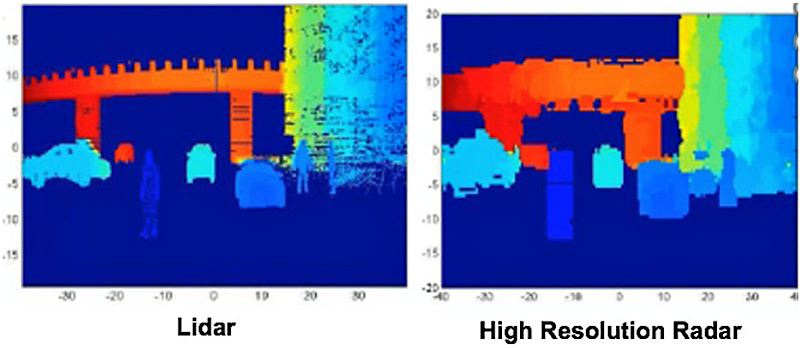
\includegraphics[width=\textwidth]{lidar-radar.png}
  \captionbelow[Vergleich Lidar und Radar Umgebungsscan]{Vergleich Lidar und Radar Umgebungsscan. (\cite{lidar-radar})}
  \label{lidar-radar}
\end{figure}

In den Fahrzeugen von Waymo, einem Tochterkonzern von Google's Mutterkonzern Alphabet, sind drei \acs{Lidar}-Scanner auf dem Dach der Fahrzeuge verbaut (siehe \ref{waymo-lidar}). Dazu gehören ein Kurzstrecken-\acs{Lidar} für den unmittelbaren Bereich um das Fahrzeug, ein Langstrecken-\acs{Lidar}, der auch aus mehreren hundert Metern Entfernung und voller Geschwindigkeit feine Signale, wie Handbewegungen, erkennen kann sowie einem hoch auflösenden \acs{Lidar}, welcher Millionen Laserimpulse pro Sekunde aussenden kann, um ein detailliertes Bild der Umwelt zu erzeugen. \vgl{waymo-lidar} In autonomen Fahrzeugen wird \acs{Lidar} hauptsächlich für zwei Aufgaben eingesetzt:
\begin{enumerate}
  \item{Erkennung und Bestimmung von Objekten um das Fahrzeug}
  \item{Präzise Positionsbestimmung innerhalb der Fahrspur}
\end{enumerate}
\vgl{Surden}

\begin{figure}\centering
  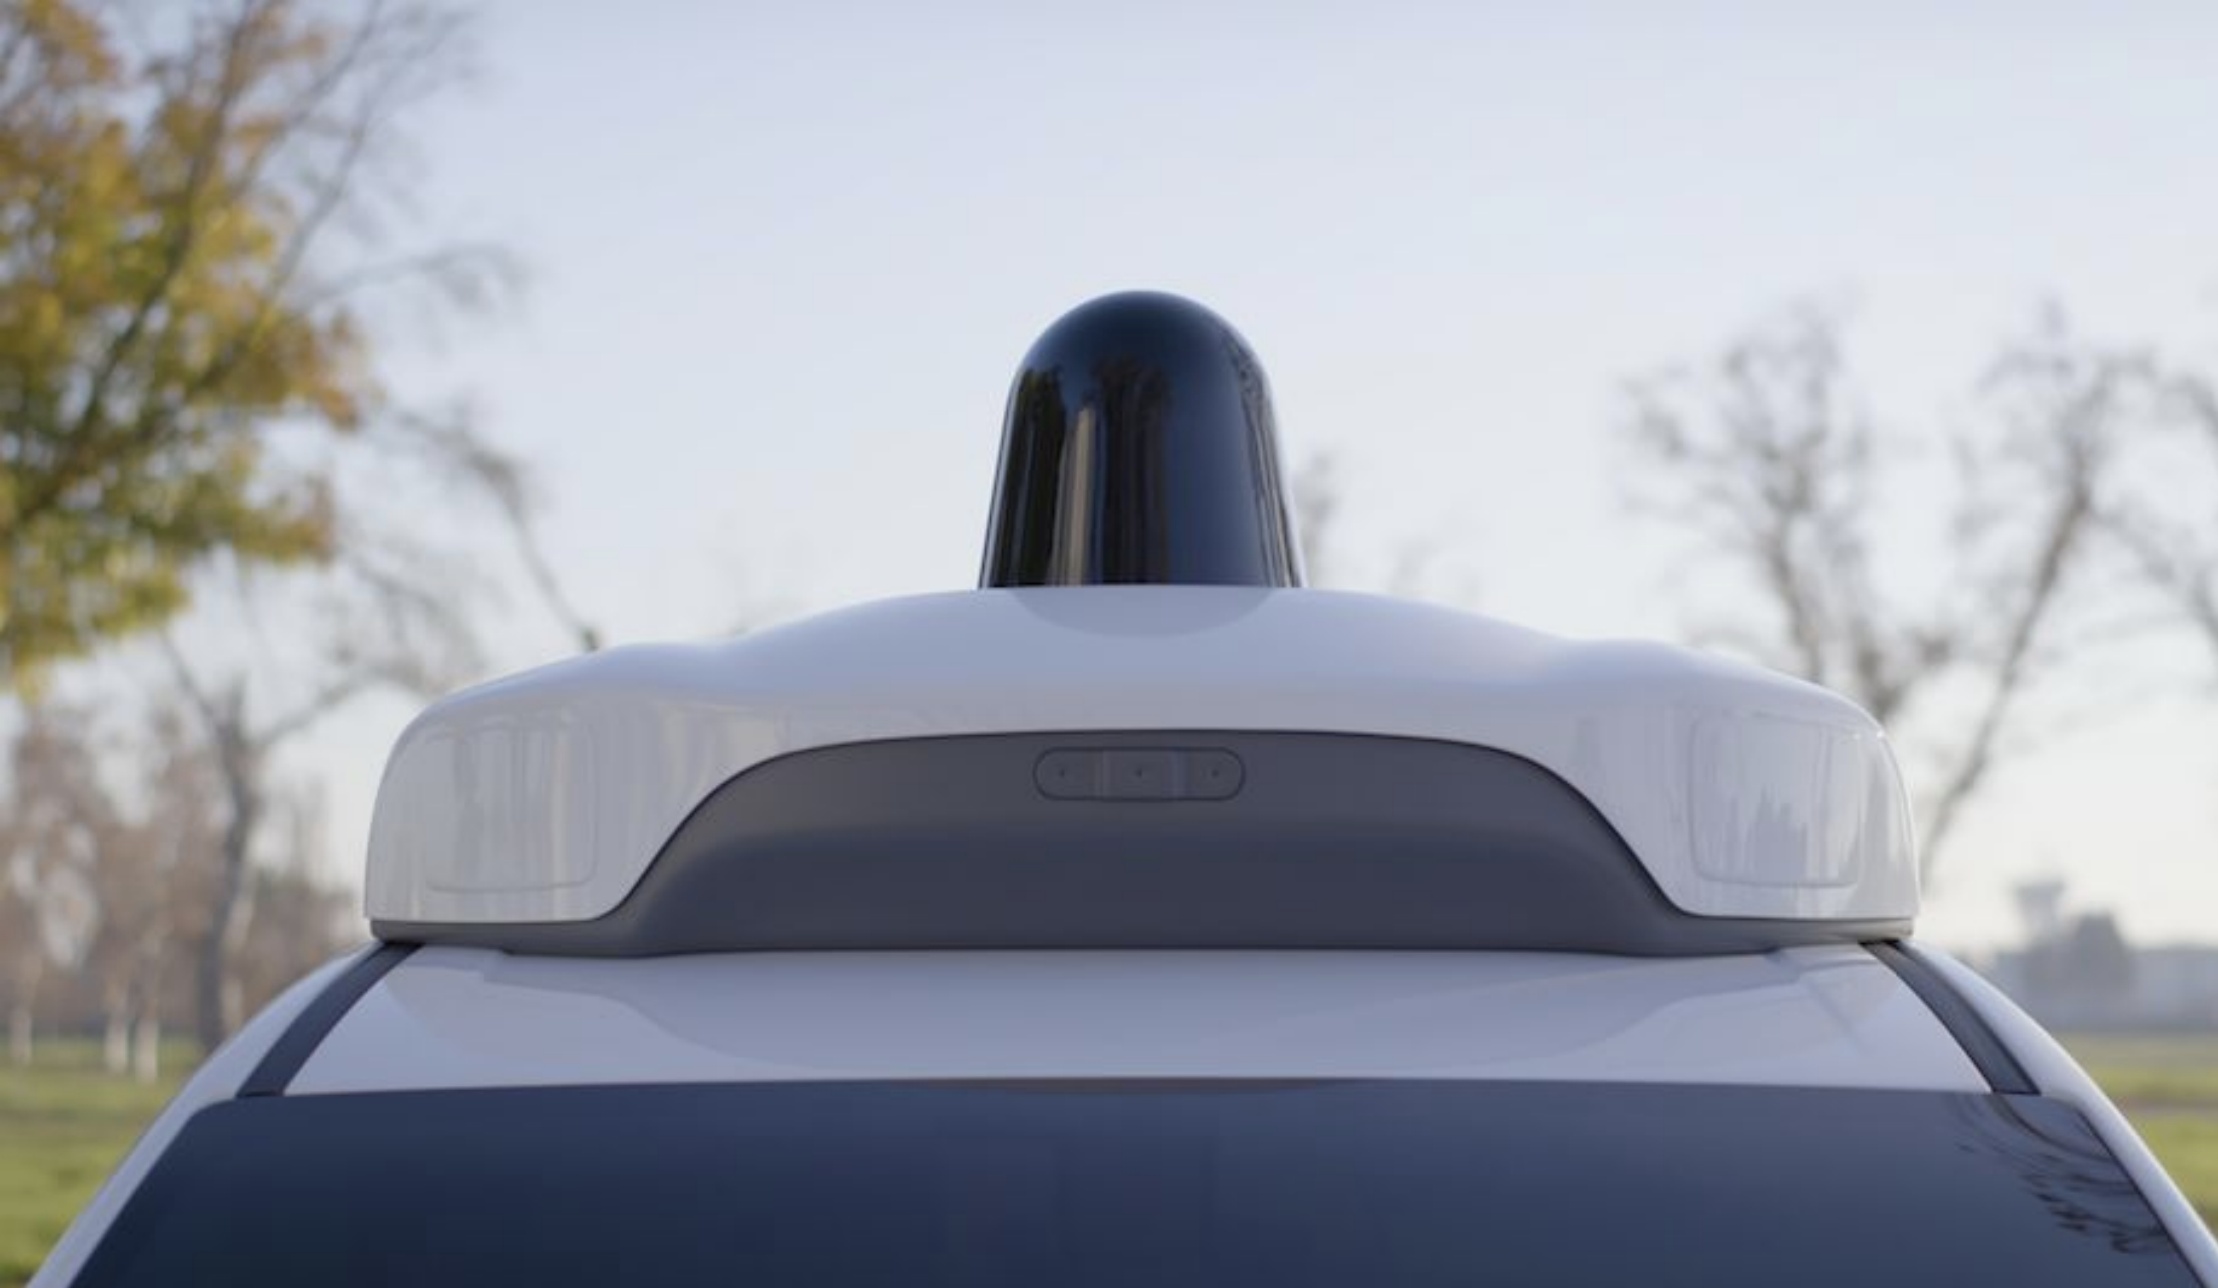
\includegraphics[width=\textwidth]{waymo-lidar.png}
  \captionbelow[Lidar-Scanner auf einem autonomen Fahrzeug von Waymo]{Lidar-Scanner auf einem autonomen Fahrzeug von Waymo. (\cite{waymo-lidar})}
  \label{waymo-lidar}
\end{figure}

\subsection{Partikel-Filter}

Eine Möglichkeit, um mittles \acs{Lidar}-Scannern die Position von Fahrzeugen bestimmen zu können, ist mittels Partikel-Filtern (auch Monte-Carlo-Lokalisierung). Hierfür wird auch eine annotierte digitale Karte (siehe \ref{maps}) benötigt, um vermessene Punkte mit den auf der Karte gespeicherten Objekten zu vergleichen.

\begin{enumerate}
  \item{Zuerst werden auf der Karte eine hohe Anzahl an sogenannten Partikeln verteilt. Jeder Partikel stellt eine mögliche Position des Fahrzeugs dar. Anfangs erhalten alle Partikel dieselbe Gewichtung (da die Position des Fahrzeugs gänzlich unbekannt ist), was bedeutet, dass alle Partikel die gleiche Wahrscheinlichkeit aufweisen, die korrekte Position darzustellen.}

  \item{Währrend sich das Fahrzeug bewegt, schickt es laufend Daten wie Geschwindigkeit und Winkel an den Fahrzeugcomputer. Jeder Partikel wird nun um dieselbe Distanz und in dieselbe Richtung wie das Fahrzeug bewegt, dieser Schritt nennt sich \textit{Prognose-Schritt}}.

  \item{Nun kommt der \textit{Vermessungsschritt}. Das Fahrzeug benutzt seine \acs{Lidar}-Scanner}, um die Distanzen zu den auf der Karte notierten markanten Punkten, zu vermessen. Jetzt werden für jeden Partikel ebenfalls die Distanzen zwischen dem Partikel und den markanten Punkten vermessen und anschließend mit den Vermessungen des Fahrzeugs verglichen. Partikel, die sich näher am Fahrzeug befinden, bekommen eine höhere Gewichtung zugewiesen.

  \item{Partikel, die unter eine gewisse Wahrscheinlichkeitsschwelle fallen, werden nun gelöscht und der Prozess ab Schritt 2 wird wiederholt.}
\end{enumerate}

Durch die ständige Wiederholung dieser Schritte ist es dem Fahrzeugcomputer möglich, dauerhaft die akurate Position des Fahrzeugs zu berechnen.
\vgl{particle-filter}

\subsection{BLMR-Methode}

Bei einer weiteren Möglichkeit, Fahrzeuge präzise zu lokalisieren, scannen \acs{Lidar}-Geräte Straßenmarkierungen, indem sie die Straßenoberfläche auf unterschiedliche Reflexionsvermögen (aufgrund weißer Markierungen) untersuchen und speichern die erfassten Daten in einer Datei namens \acs{BLMR} (\acl{BLMR}). In der \acs{BLMR} werden stets die Leit- und Randliniendaten der letzten \SI{240}{\meter} gespeichert, diese werden laufend mit den zuvor erstellten annotierten digitalen Karten (siehe \ref{maps}) abgeglichen, wodurch der Standort bestimmt werden kann. \vgl{self-localization}

Auch bei dieser Methode können sich die Sensoren automatisch an anderen markanten Punkten wie Straßenschildern, Ampelanlagen, Gebäuden oder Bäumen orientieren, sollten keine Straßenmarkierungen vorhanden sein. Wichtig ist nur, dass es sich bei den Objekten um Dinge handelt, deren Standort sich nicht ändert und die eindeutig für \acs{Lidar}-Scanner erkennbar sind.

\subsection*{Nachteile von Lidar}

Trotz der Vorteile wie der hohen Genauigkeit oder auch großen Reichweite haben auch \acs{Lidar}-Scanner Nachteile. Einer davon ist der Preis, besonders Geräte für große Distanzen sind teuer, da hierfür Laser mit einer Wellenlänge von \vgl{imu-def}\SI{1550}{\nano\meter} benötigt werden, um für Menschen nicht schädlich zu sein. Um solche Laserstrahlen wiederum empfangen zu können, sind Empfänger aus \ac{InGaAs} notwendig, da Siliziumempfänger, welche um ein Vielfaches günstiger als solche aus \ac{InGaAs} sind, keine Laserstrahlen mit \SI{1550}{\nano\meter} Wellenlänge erkennen können. \vgl{wired} Durch jahrelange Entwicklung und ständig steigenden Produktionszahlen hat es Waymo mittlerweile geschafft, die Kosten für einen \acs{Lidar}-Scanner von \$\,\num{75000} um 90\,\% auf \$\,\num{7500} zu reduzieren. \vgl{waymo-medium}

Ein weiterer Nachteil ist die Abhängigkeit von gutem Wetter. Schnee, Regen oder Nebel reflektieren das Licht, was zur Folge hat, dass das Fahrzeug fälschlicherweise Hindernisse erkennt, welche in Wirklichkeit nur Regentropfen oder Schneeflocken sind. Dieser Bereich unterliegt aktuell noch weiteren Forschungen, Ford hat jedoch schon einen Algorithmus entwickelt, der dieses Problem beheben soll. Dabei werden die empfangenen Laserstrahlen genau auf ihre Eigenschaften untersucht, etwa ob sich ein Objekt, von welchem der Laser reflektiert wird, zweimal an der selben Stelle befindet, was bei Regentropfen nicht der Fall ist.
\vgl{ford-qz}


\section{Positionsbestimmung ohne Lidar am Beispiel von Tesla}\label{section-2-3}

Anhand Teslas Fahrerassistenzsystem, dem sogenannten \enq{Autopilot}, lässt sich sehen, dass eine präzise Positionsbestimmung auch ohne \acs{Lidar}, sondern nur mit einer Kombination aus Ultraschallsensoren, Kameras und einem \acs{Radar}, möglich ist. Teslas aktuelle Autopilot 2.0 Hardware, mit der autonomes Fahren auf \ac{SAE}-Level 5 möglich sein soll, umfasst zwölf Ultraschallsensoren, acht Kameras sowie einen \acs{Radar} (siehe \ref{autopilot-hardware}).

\begin{figure}\centering
  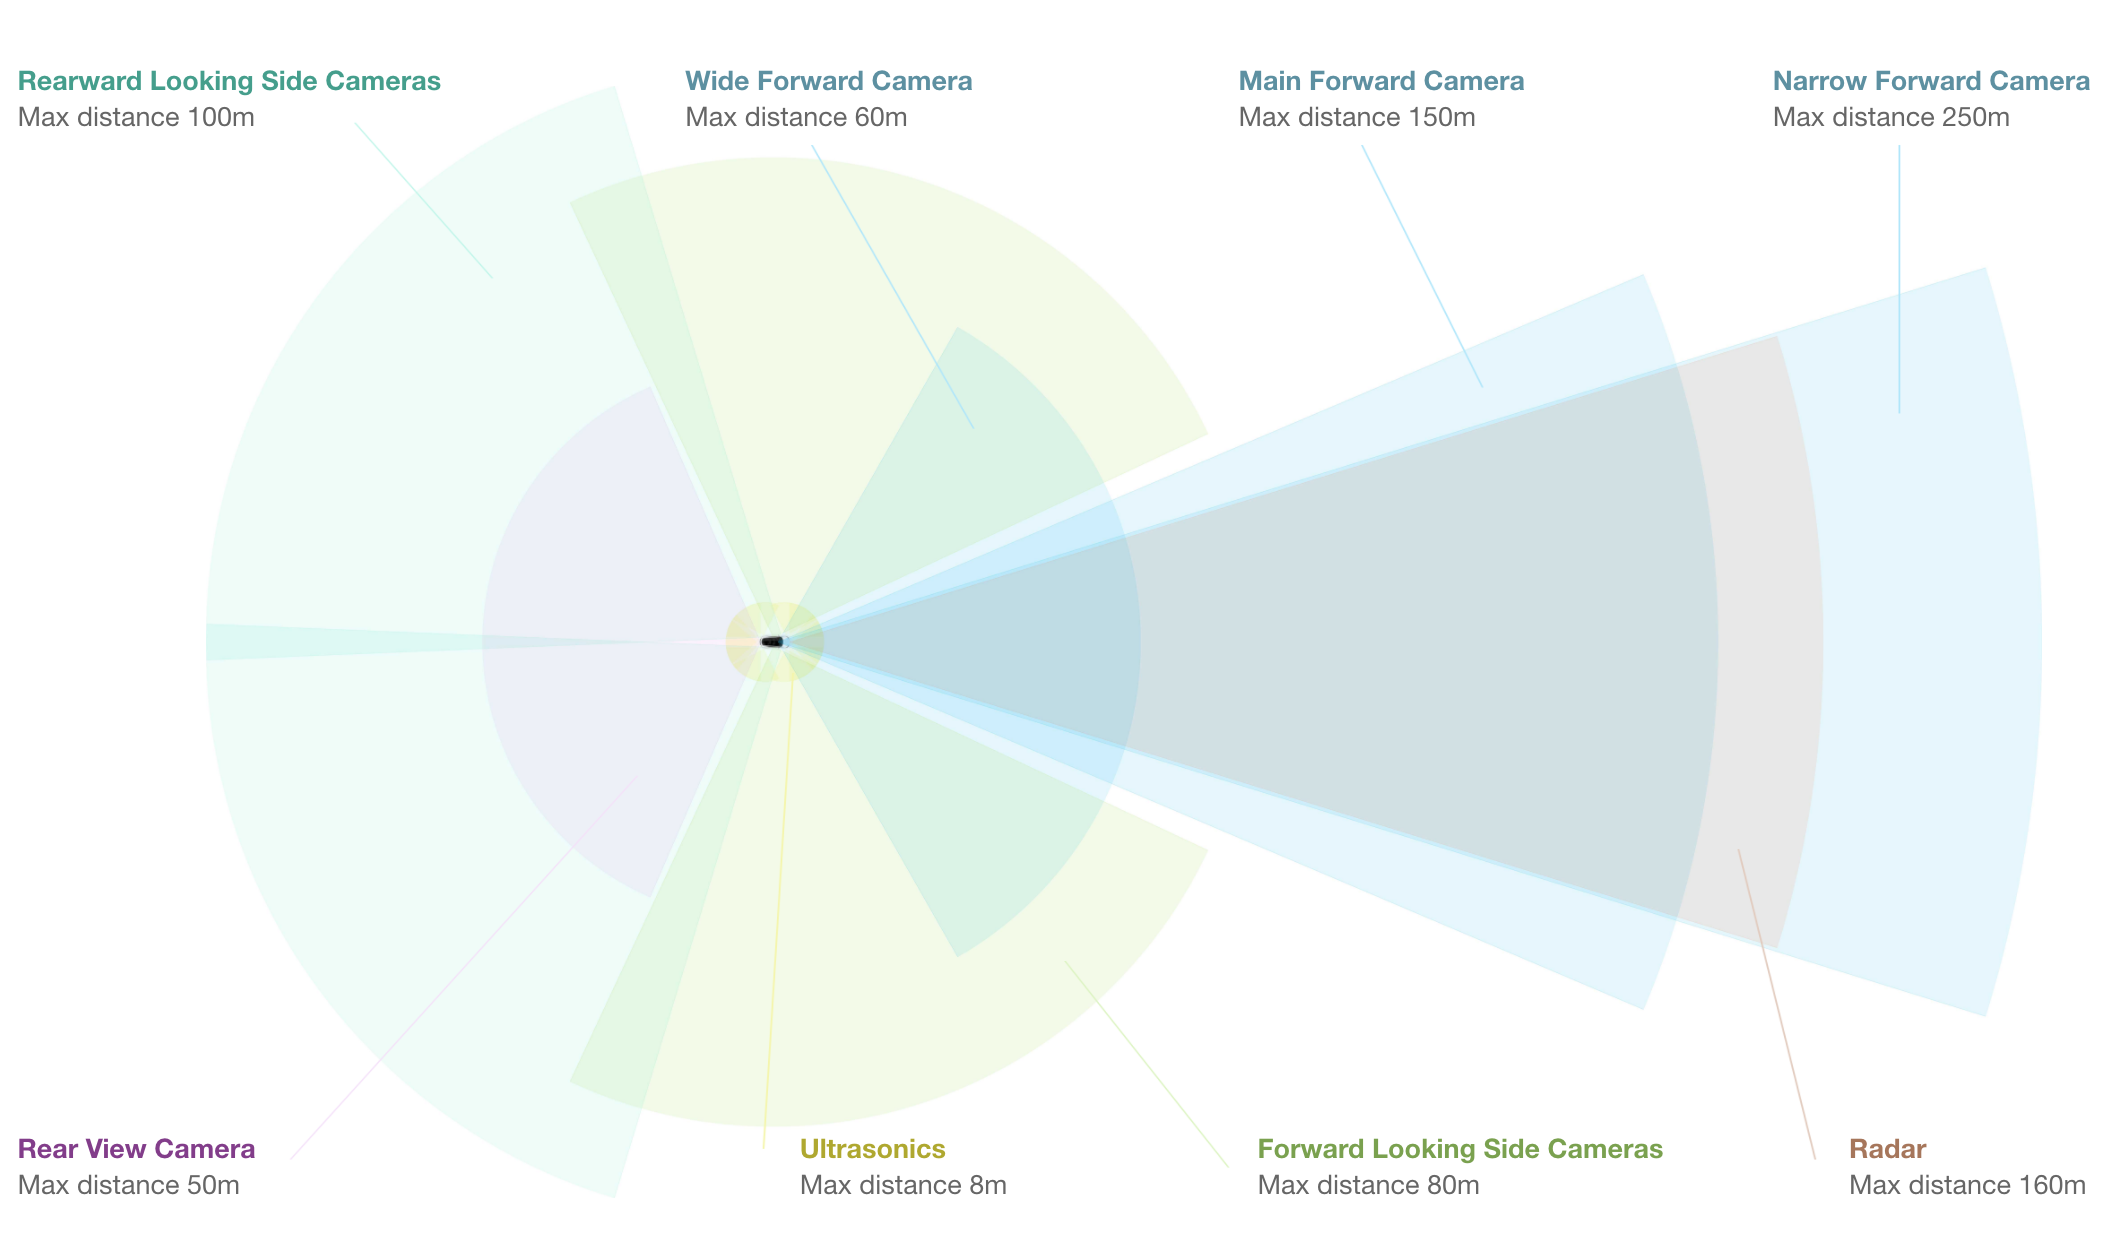
\includegraphics[width=\textwidth]{autopilot-hardware.png}
  \captionbelow[Tesla Autopilot 2.0 Hardware]{Tesla Autopilot 2.0 Hardware. (\cite{tesla-autopilot})}
  \label{autopilot-hardware}
\end{figure}

\noindent Elon Musk, CEO von Tesla, sagte in einem Konferanzanruf mit der Presse 2016: \zit{elon-musk}{We are confident that we can use the radar to look beyond the car in front of you by bouncing the radar signal off the road and around the car. \elp{}
So even if there’s something that was obscured directly both in vision and radar, we can use the bounce effect of the radar to look in front of that car and still brake.
It takes things to another level of safety.}

Mikrowellen eines \acs{Radar} ist es im Gegensatz zu Licht möglich, vom Boden zurückzuprallen. Dieser Umstand ermöglicht dem \acs{Radar}, unter einem vorherfahrenden Fahrzeug hindurch zu sehen und Gefahrensituationen frühzeitig zu erkennen, wodurch eventuell notwendige Notbremsmanöver rechtzeitig eingeleitet werden können. \vgl{ars-technica}

Außerdem verbaut Tesla in seinen Fahrzeugen keine \acs{Lidar}-Systeme, weil das Problem der Reflexion bei Regen, Nebel und Schneefall nicht besteht. Mikrowellen, wie die des \acs{Radar}, können diese Niederschläge durchdringen, wodurch keine fehlerhaften Erkennungen von Objekten entstehen, die gar nicht existieren. \vgl{ars-technica}

\chapter{Aktueller Entwicklungsstand}

Dieses Kapitel soll einen Überblick über die aktuellen Entwicklungen im Bereich der Technologien, die für autonomes Fahren, speziell für die Positionsbestimmung, benötigt werden, vermitteln. Außerdem werden einige Projekte behandelt, die es sich zur auf Aufgabe gemacht haben, autonomes Fahren auf die weltweiten Straßen zu bringen.


\section{\acs{Lidar}-Entwicklung}

Die Entwicklung von Lidar-Scannern ist schreitet schneller voran als je zuvor. Eines der zahlreichen Unternehmen, die sich an der Entwicklung beteiligen, ist Ouster, ein US-amerikanisches Unternehmen, dessen Ziel es ist, ein massentaugliches Lidar-System zu einem relativ erschwinglichen Preis auf den Markt zu bringen. \Vgl{ouster-web}

Derzeit bietet Ouster seinen \acs{Lidar}-Scanner \emph{OS-1} in drei verschiedenen Varianten mit 16, 64 oder 128 Kanälen an. Eine höhere Anzahl an Kanälen resultiert in einer höheren Auflösung, das Modell mit 16 Kanälen bietet eine Abtastrate von \num{327680} Punkten pro Sekunde, bei 128 Kanälen sind Abtastraten von \num{2621440} Punkten pro Sekunde möglich. Die Preise liegen zwischen \num{3500} und \num{18000} US-Dollar, für Non-Profit-Unternehmen und wissenschaftliche Einrichtungen gibt es zudem Vergünstigungen von bis zu 45 Prozent. \Vgl{ouster-web}


\section{Nvidia DRIVE Localization}

Auf der jährlich in Las Vegas stattfindenden Consumer Electronics Show (CES) hat Nvidia, ein Unternehmen, welches eigentlich für High-End Grafikkarten bekannt ist, im Jänner 2019 eine offene Plattform namens \emph{Nvidia DRIVE Localization} vorgestellt. Das System basiert auf Nvidias hauseigenem, speziell für autonomes Fahren etwickelten Prozessor \emph{Nvidia DRIVE Xavier}, bei dem es sich um einen sogenannten \ac{SoC} handelt, welcher einen Deep Learning Accelerator und eine CUDA-Engine\footnote{\zit{cuda}{CUDA ist eine NVIDIA Architektur für parallele Berechnungen, die die Rechenleistung des Systems durch Nutzung der Leistung des Grafikprozessors deutlich steigern kann.}} beinhaltet. \Vgl{nvidia-drive}

Das System kommt dabei ohne jegliche \acs{Lidar}- oder \acs{Radar}-Scanner aus, es greift lediglich auf ein \ac{GNSS}, eine \ac{IMU} und den Tachometer des Fahrzeugs zurück. Neurale Netzte analysieren die Daten in Echtzeit und können verschiedenste Straßenmerkmale selbst in schlechten Wetterbedingungen auslesen. Diese Anforderungen können nur durch ernorme parallele Recheleistung, welche vom Xavier \ac{SoC} zur Verfügung gestellt wird, bewältigt werden. \Vgl{nvidia-drive}


\section{Waymo}

Waymo ist ein Schwesterunternehmen von Google und führt das im Jahr 2009 gegründete Projekt \emph{Google Driverless Car} fort. 2015 fand die erste, voll autonome Fahrt auf öffentlichen Straßen in Austin statt. Im Oktober 2018 erreichte Waymo den Meilenstein von 10 Millionen zurückgelegten Meilen (ca. 16 Millionen Kilometer) in ihrer Flotte von autonomen Fahrzeugen.

Am 5.\ Dezember 2018 startete Waymo ein kommerzielles Taxi-Service namens \emph{Waymo One} in vier Vororten von Phoenix, Arizona. Die autonomen Fahrzeuge werden derzeit noch von einem \enq{Sicherheitsfahrer} begleitet, der im Fall einer Fehlfunktion der autonomen Systeme, die Kontrolle über das Fahrzeug übernehmen kann \vgl{waymo-taxiservice}{}. Bereits seit 2017 bis zum Start von \emph{Waymo One} lief das sogenannte \emph{Early rider program}, an dem ausgewählte Bewohner des Ballungsraums von Phoenix teilnehmen konnten, um kostenlose Taxifahrten zu erhalten. Das Feedback der Teilnehmer trug zur Weiterentwicklung der autonomen Fahrzeuge bei.
\Vgl{waymo-website}


\section{Uber}

Auch der Fahrtendienst Uber hat im Februar 2015 bekanntgegeben, eine Flotte an autonomen Fahrzeugen aufzubauen um diese für Testfahrten zu benützten. Nach ersten Tests ist Pittsburgh, die jedoch nach einiger Zeit aufgrund von Differenzen mit dem Bürgemeister der Stadt nach San Francisco verlegt wurden. Seit 2017 finden auch, ebenso wie bei Waymo, Tesfahrten im benachbarten Arizona statt. \Vgl{uber-tech-radar}

Bei einem Unfall im März 2017 in Tempe, Arizona wurde eine Frau von einem selbstfahrenden Uber-Fahrzeug, einem Volvo XC90, erfasst und dabei tödlich verletzt. Die Frau schob ihr Fahrrad über die vierspurige Straße, trotz Dunkelheit wurde sie aber von den zahlreichen Sensoren des Fahrzeug bereits sechs Sekunden vor dem Unfall erkannt. Das System war aber verwirrt, zuerst erkannte es die Frau als unbekanntes Objekt, dann als Fahrzeug und zuletzt als Fahrrad, dessen Pfad es nicht vorhersagen konnte. Nur 1,3 Sekunden vor dem Zusammenstoß erkannte das System, dass eine Notbremsung nötig war, führte diese jedoch nicht durch, da das automatische Notbremssystem deaktiviert war. Der Sicherheitsfahrer, der gerade auf einen Bildschirm des autonomen Systems schaute, konnte nicht mehr rechtzeitig Bremsen, wodurch das Fahrzeug ungebremst mit ungefähr \SI[per-mode=symbol]{60}{\kilo\metre\per\hour} auf das Opfer zufuhr. Nach dem Unfall wurden alle autonomen Testfahrten von Uber vorläufig eingestellt, nach rund einem Jahr wurden die Tests wieder fortgeführt.
\Vgl{uber-unfall}


\section{Tesla}

Tesla ist, ebenso wie Waymo, ein im Silicon Valley ansässiges Unternehmen mit folgendem selbst ernannten Ziel: \zit{tesla-about}{Die Beschleunigung des Übergangs zu nachhaltiger Energie.} Um dieses Ziel erreichen zu können, stellte Tesla im Jahr 2008 den Roadster vor, einen zweisitzigen Sportwagen, der die Finanzierung der Premium-Limousine Model S sicherte. Besondere Merkmale sind die größte Reichweite unter Elektrofahrzeugen und eine Beschleunigung von 0 auf 100 \si[per-mode=symbol]{\kilo\metre\per\hour} in 2,7 Sekunden. Derzeit läuft die Auslieferung der im Vergeleich zum Model S kompakteren Limousine Model 3, welches durch einen Grundpreis von \num{35000} US-Dollar die Verbreitung von Elektrofahrzeugen weiter vorantreiben soll.
\Vgl{tesla-about}

Teslas Fahrzeuge zählen außerdem zu den sichersten der Welt. Wie in \ref{safety-chart} zu sehen, sind von allen seit 2011 von der \ac{NHTSA} getesteten Fahrzeuge, die drei mit der niedrigsten Wahrscheinlichkeit von Verletzungen, alle von Tesla hergestellt. Das Model 3 hat hierbei einen besonders niedrigen Wert von nur 5,7 Prozent. Dieser Wert errechnet sich durch den \enq{Vehicle Safety Score} von 0,38 der mit der von der \ac{NHTSA} angegebenen Basiswahrscheinlichkeit von 15 Prozent multipliziert wird. \Vgls[40038]{nhtsa-baseline}{model-3-score}

\begin{figure}\centering
  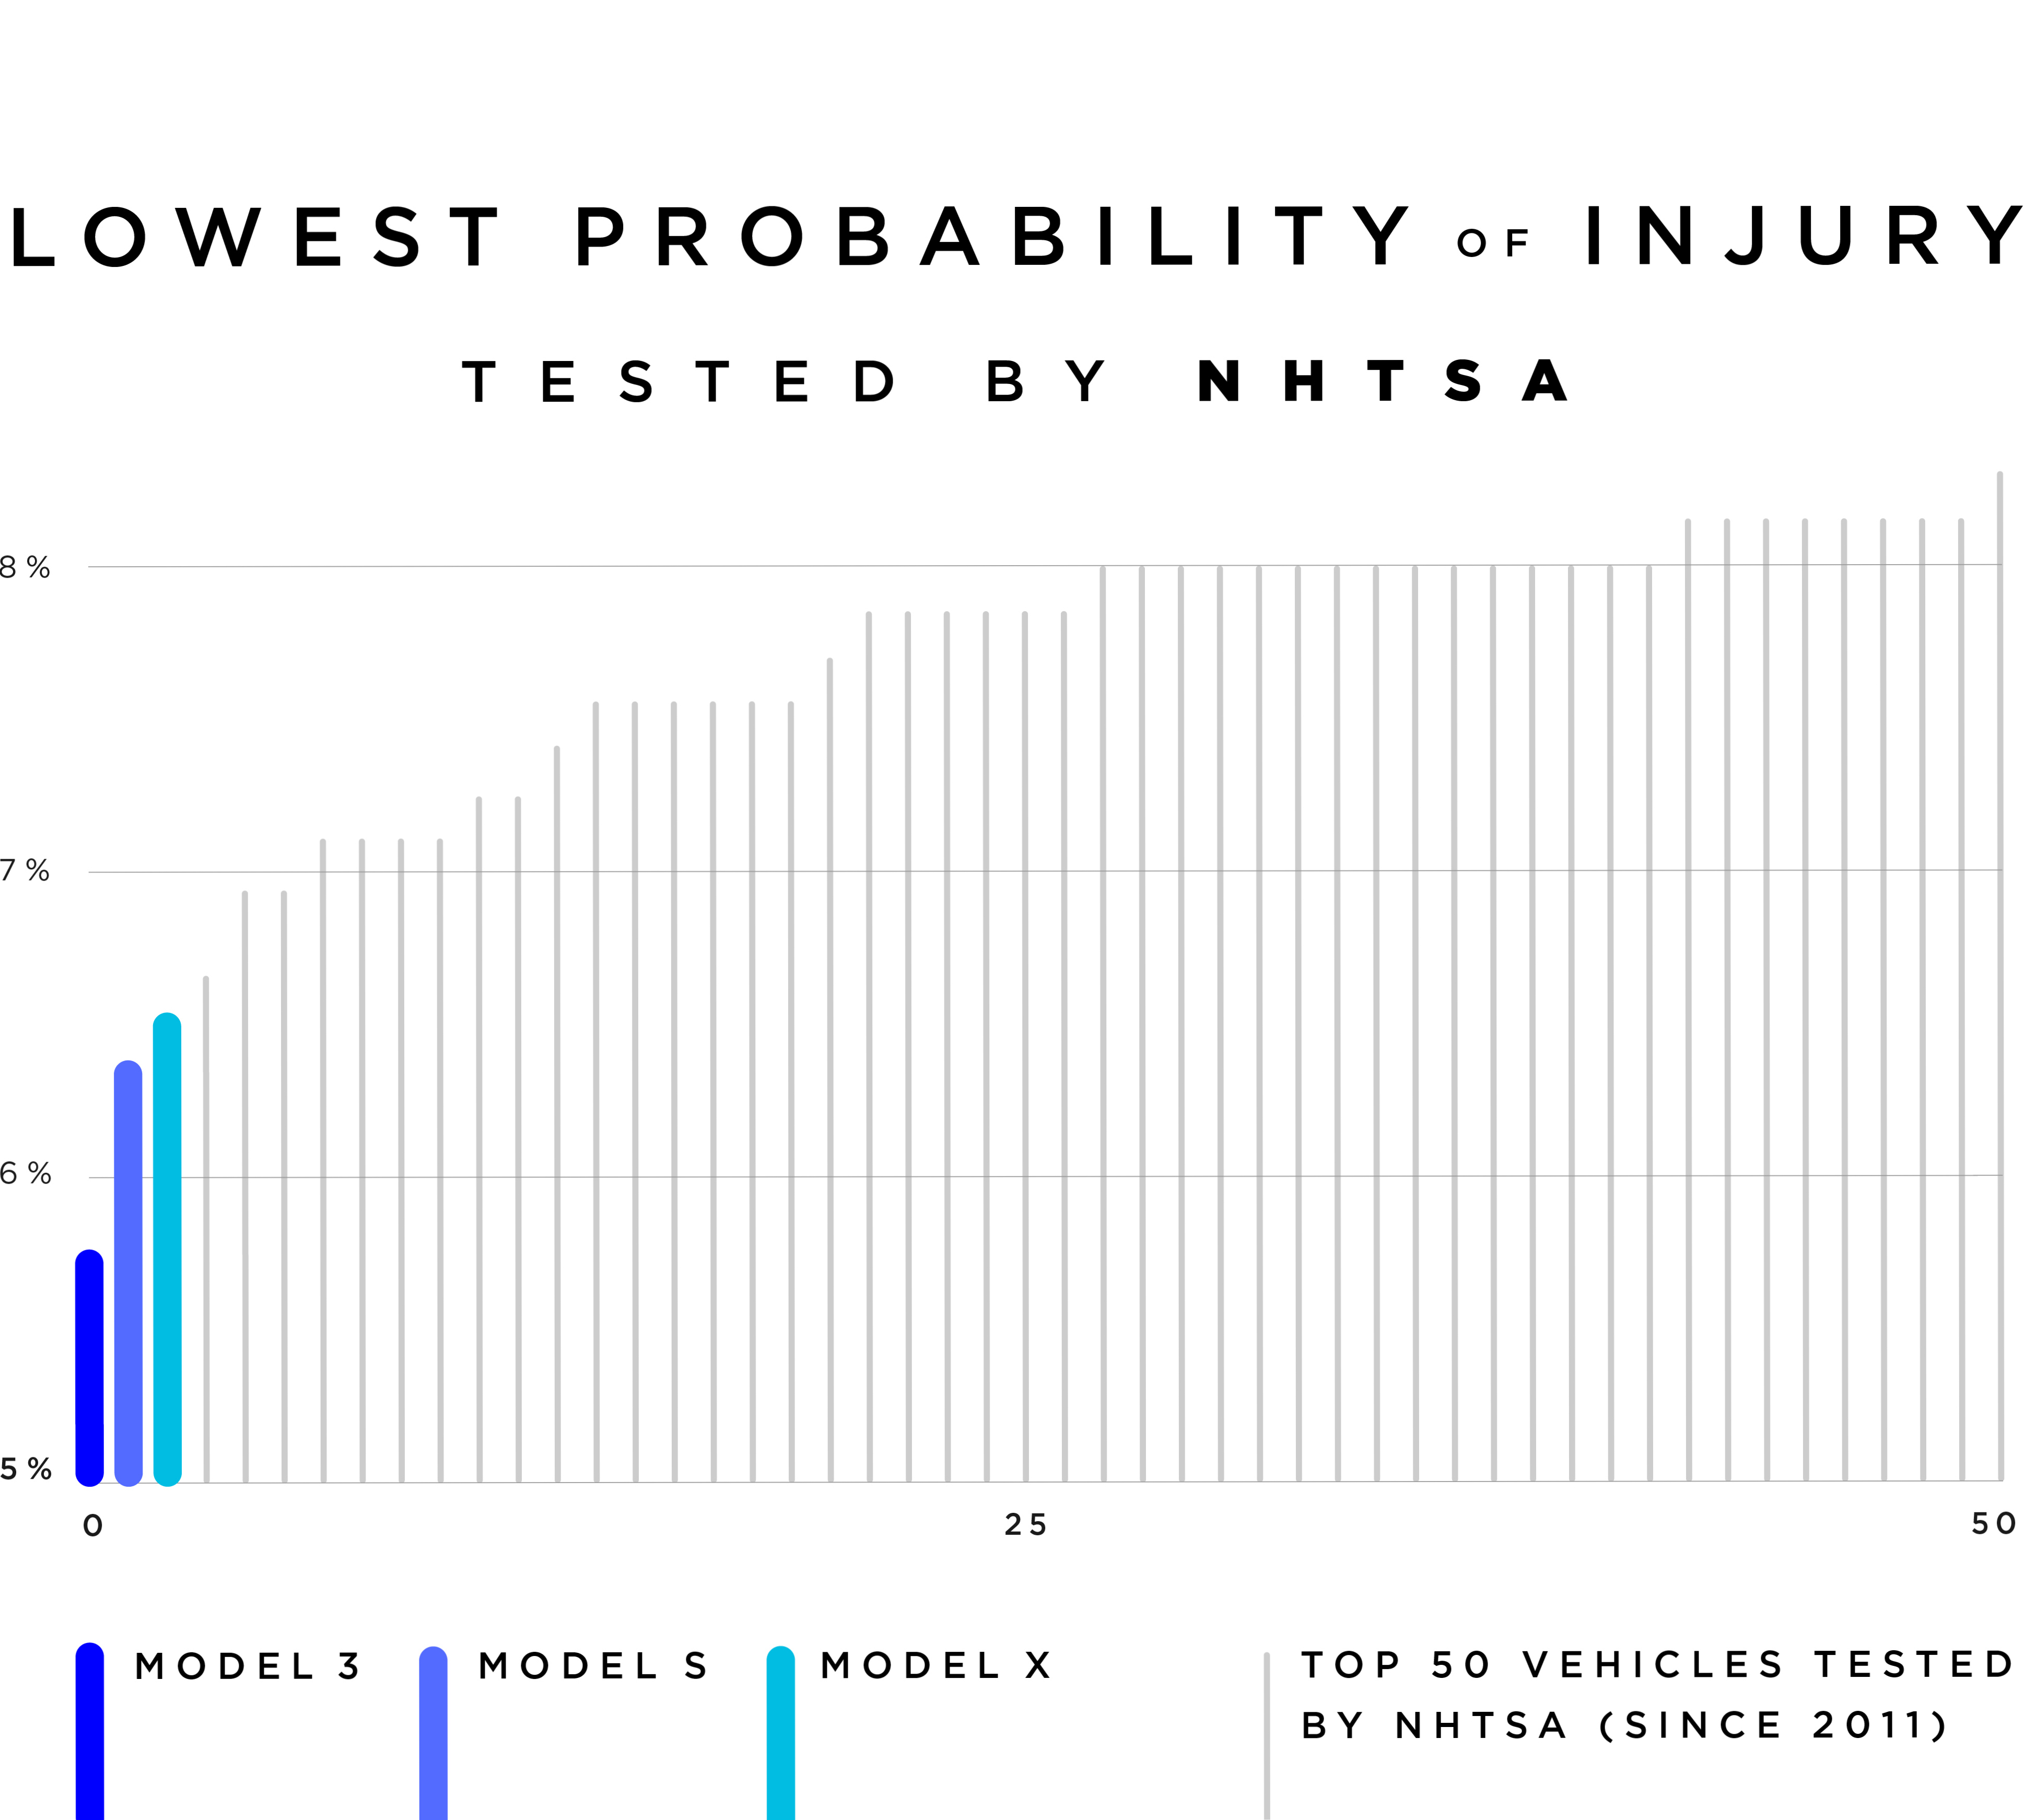
\includegraphics[width=\textwidth]{safety-chart.jpg}
  \captionbelow[Niedrigste Wahrscheinlichkeit von Verletzungen. Getestet von der \ac{NHTSA}. Bildquelle: \fullcite{tesla-safety}]{Niedrigste Wahrscheinlichkeit von Verletzungen. Getestet von der \ac{NHTSA} (\cite{tesla-safety})}
  \label{safety-chart}
\end{figure}

Weiters ist Tesla für seinen bereits in \ref{section-2-3} behandelten Autopilot. Am 27.\ November haben Teslas Fahrzeuge eine Milliarde Meilen (ca. 1,6 Milliarden Kilometer) mit aktiviertem Autopilot zurückgelegt. Das entspricht etwa 10 Prozent aller von Teslas Fahrzeuges weltweit gefahrenen Meilen, wobei hierbei auch Fahrzeuge ohne Autopilot-Hardware bzw. solche mit Hardware, jedoch ohne der notwendigen kostenpflichtigen Aktivierung des Assistenzsystems miteingerechnet werden. \Vgl{electrek-one-billion}


\section{Wiener Linien}

Im Frühjahr 2019 soll die erste autonome Buslinie Wiens in der Seestadt in Betrieb gehen. Das Projekt namens \emph{auto.Bus - Seestadt} durchläuft derzeit intensive Testfahrten auf geschlossenem Gelände. Bei dem Bus handelt es sich um einen vollelektrischen Kleinbus (siehe \ref{bus-seestadt}), der Platz für bis zu zehn Fahrgäste und einen Operator bietet. Der Operator ist derzeit noch aus sicherheitsgründen notwendig, er überwacht den Bus und kann im Ernstfall ins Geschehen eingreifen. \Vgl{wiener-linien}

\begin{figure}\centering
  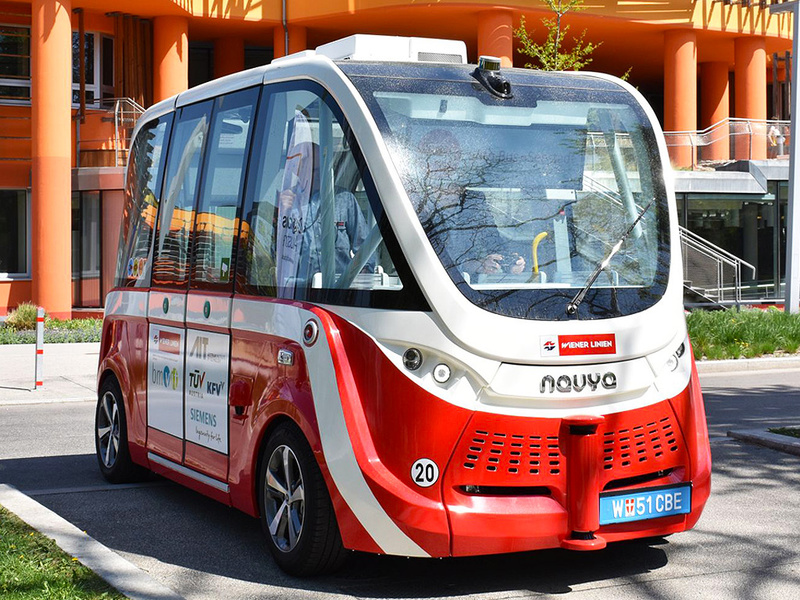
\includegraphics[width=\textwidth-1cm]{bus-seestadt.jpg}
  \captionbelow[Elektrischer Kleinbus der Wiener Linien. Bildquelle: \fullcite{wiener-linien}]{Elektrischer Kleinbus der Wiener Linien (\cite{wiener-linien})}
  \label{bus-seestadt}

  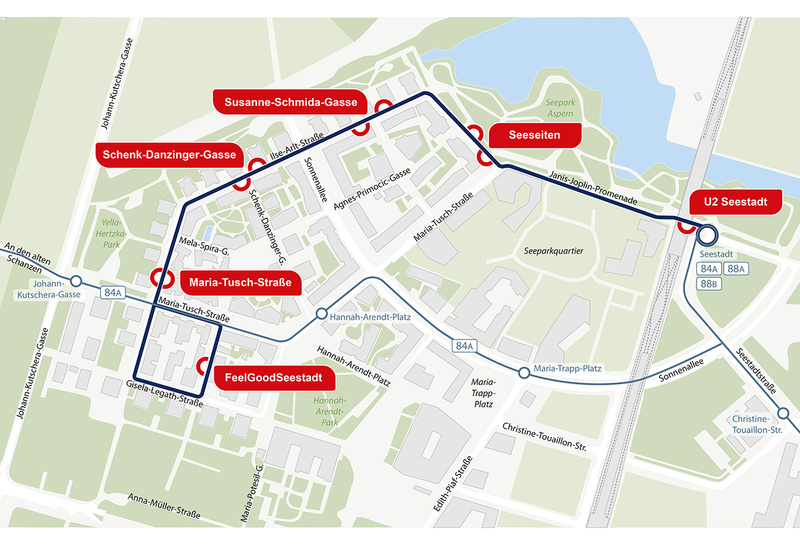
\includegraphics[width=\textwidth-1cm]{bus-seestadt-karte.jpg}
  \captionbelow[Geplante Route der autonomen Buslinie. Bildquelle: \fullcite{wiener-linien}]{Geplante Route der autonomen Buslinie (\cite{wiener-linien})}
  \label{bus-seestadt-karte}
\end{figure}

Die geplante Route ist in \ref{bus-seestadt-karte} dargestellt, sie ist 2 \si{\kilo\metre} lang und bedient sechs Stationen in der Seestadt. Die Beförderung auf der Linie ist kostenlos. Da es sich um einen Testbetrieb handelt, ist der Transport von Kinderwägen und Rollstühlen rechtlich nicht erlaubt.
\Vgl{wiener-linien}


\section{Aktionspaket des Bundesministeriums für Verkehr, Innovation und Technologie}

Das \ac{bmvit} veröffentliche im November 2018 sein \emph{Aktionspaket Automatisierte Mobilität. 2019 -- 2022}, in dem Österreichs Ziele und Maßnahmen zur Verbreitung von autonomem Fahren dargelegt werden.

Durch eine Novelle des Kraftfahrgesetztes im Jahr 2016, wurden die rechtlichen Rahmenbedingungen geschaffen, um \enq{ALP.Lab} (Austrian Light Vehicle Proving Region for Automated Driving), Österreichs erste Testumgebung für autonome Fahrzeuge, in der Steiermark zu errichten. Durch Erstellung der Verordnung zum automatisierten Fahren konnten außerdem erstmals Test auf öffentlichen Straßen durchgeführt werden \vgl{automat-fahr-v}{}. Hierbei werden insbesondere Autobahnpiloten mit automatischem Spurwechsel, selbstfahrende Heeresfahrzeuge und autonome Kleinbusse getestet.
\Vgl[10]{bmvit}

Das \ac{bmvit} strebt einen \zit[23]{bmvit}{verkehlich sinnvollen und effizienten Einsatz automatisierter Mobilität sowie die Stärkung der Wettbewerbsposition Österreichs} an. In erster Linie gehe es allerdings laut Aktionsplan um \zit[23]{bmvit}{lebenswerte öffentliche Räume.} Diese Punkte will die Regierung besonders durch Testen und Pilotieren erreichen, wobei der Nutzer Mittelpunkt dieser Tests sein soll. Letztendlich muss nämlich der Verkehr für alle die an ihm teilnehmen eines werden: sicherer. Insbesondere schwächere Verkehrsteilnehmer wie Radfahrer oder Fußgänger sollen in ihrer Sicherheit gestärkt werden.

Ein weiteres wichtiges Anliegen ist die Reduktion der \ce{CO2}-Emissionen im Verkehrssektor, bis 2050 soll Österreichs Verkehr vollständig \ce{CO2}-neutral werden. Das ist nicht nur durch den Einsatz elektrischer Fahrzeuge erreichbar, sondern auch durch autonome Mobilität. Die Notwendigkeit eines eigenen Fahrzeuges ist durch autonome Taxis, die rund um die Uhr von jedermann verwendet werden können, nicht mehr so hoch wie heute.
\Vgl[24]{bmvit}


% 20180120T2131 Leonard Michlmayr

%% Einige Filter für die Einträge im Literaturverzeichnis
\defbibfilter{online}{( type=online or subtype=online )}
\defbibfilter{interview}{type=interview or subtype=interview}
\defbibfilter{onlinetext}{( type=online or subtype=online and not ( type=video
  or type=audio ) )}
\defbibfilter{offline}{not ( type=online or subtype=online )}
\defbibfilter{print}{not ( type=online or subtype=online or type=video or
  type=audio or type=interview or subtype=interview )}
\defbibfilter{offlinevideo}{type=video and not subtype=online}
\defbibfilter{offlineaudio}{type=video and not subtype=online}
\defbibfilter{nurAusSekundaerliteratur}{category=quotee and not category=primary}
\defbibfilter{nichtNurAusSekundaerliteratur}{category=quoter or category=primary}

% TODO: die Untergliederung des Literaturverzeichnisses den eigenen
% Bedürfnissen anpassen.
\printbibheading[heading=bibintoc,title=Literaturverzeichnis]\label{Lit}
\printshorthands[heading=subbibintoc]
\printbibliography[heading=subbibintoc,title={Print-Quellen},filter=print,filter=nichtNurAusSekundaerliteratur]
\printbibliography[heading=subbibintoc,title={Audio-Quellen},filter=offlineaudio,filter=nichtNurAusSekundaerliteratur]
\printbibliography[heading=subbibintoc,title={Video-Quellen},filter=offlinevideo,filter=nichtNurAusSekundaerliteratur]
\printbibliography[heading=subbibintoc,title={Internet-Quellen},filter=online,filter=nichtNurAusSekundaerliteratur]
\printbibliography[heading=subbibintoc,title={Sekundärzitate},filter=nurAusSekundaerliteratur]
\printbibliography[heading=subbibintoc,title={Interviews},filter=interview]

\listoffigures
\begingroup
\let\clearpage\relax
\listoftables
\endgroup
\appendix
\chapter{Akronyme und Abkürzungen}

\begin{acronym}[XXXXXX]
  \acro{BLMR}{Back Lane Marking Registry}
  \acro{bmvit}[BMVIT]{Bundesministerium für Verkehr, Innovation und Technologie}
  \acro{GNSS}{Global Navigation Satellite System}
  \acro{GPS}{Global Positioning System}
  \acro{IMU}{Inertial Measurement Unit}
  \acro{InGaAs}{Indiumgalliumarsenid}
  \acro{Lidar}{Light detection and ranging}
  \acro{NHTSA}{National Highway Traffic Safety Administration}
  \acro{Radar}{Radio detection and ranging}
  \acro{SAE}{SAE International}
  \acro{SoC}{System-on-a-Chip}
\end{acronym}


\backmatter

%\pdfbookmark[0]{Erklärungen}{erkl}
\addchap{Erklärungen}
\section*{Selbstständigkeitserklärung}
\thispagestyle{plain}
Ich erkläre, dass ich diese vorwissenschaftliche Arbeit eigenständig
angefertigt und nur die im Literaturverzeichnis angeführten Quellen und
Hilfsmittel benutzt habe.

\vspace{2cm}\noindent Wien, \today

% TODO: Erkläre dich selbstständig selbstständig!
\vspace{2cm}\noindent\makeatletter\@AutorIn\makeatother

\vspace{2cm}\noindent

\section*{Informatikschwerpunkt}

Die vorliegende Arbeit erfüllt die Kriterien zur Abbildung des
Informatikschwerpunktes an der De La Salle Schule Strebersdorf, AHS.

\textbf{Begründung:} Die Arbeit wurde in \LaTeX{} mit entscheidenden
Kenntnissen zum Quelltext verfasst.\vspace{.5\baselineskip}

\noindent\textit{Geprüft am \ldots durch Mag. Leonard Michlmayr und Prof. Mag.
Kurt-Michael Rauch}

\end{document}
